\chapter{Luminosity  Measurement and Calibration}
\label{ch3}

Accurately measuring the luminosity delivered to the CMS experiment by the LHC is essential for various reasons. Online, the luminosity measurement provides feedback on the LHC and CMS performance and operations, including measuring trigger rates. In offline analysis, the luminosity measurement is a critical component for measuring the cross-section of observed processes or setting upper limits in searches for processes beyond the standard model.

To measure luminosity, a total of seven luminometers are used at CMS, and each of them reads out a specific quantity observed in the detector, such as hits, tracks, or clusters. The rate R measured by the luminometer is proportional to the instantaneous luminosity, $\mathcal{L}_{inst}$, with the constant of proportionality given by the visible cross-section $\sigma{vis}$ \cite{pas_18}.

\begin{equation}
R(t)=\mathcal{L}_{inst}\sigma_{vis}
\label{lumi_exp_gen}
\end{equation}

The determination of $\sigma_{vis}$ is carried out through van der Meer (vdM) scans performed with a dedicated LHC machine setup.

\section{Pixel Cluster Counting method}

The PCC method utilizes the rate of pixel clusters in the CMS pixel detector to determine the luminosity. The pixel detector's large area and low occupancy yield measurements with excellent linear response and high statistical precision. However, the statistical precision for a single 23-second period or "luminosity section" is not as high as for online luminometers due to the limited CMS trigger bandwidth available for collecting data. Nonetheless, over longer time periods, this method provides a stable and highly precise luminosity measurement. On average, the detector occupancy is less than 0.1\% \cite{pas_18}.

To obtain the mean number of pixel clusters per event, several zero-bias events are averaged. This value is given by :

\begin{equation}
\left < N_{\text{cluster}} \right > = \left < N_{\text{pixel}/\text{interaction}} \right >  \left < N_{\text{interactions}} \right > \equiv \left < N_{\text{pixel}/\text{interaction}} \right > \mu
\end{equation}

where in the last step, the average number of interactions per bunch crossing, pileup, is denoted by the symbol $\mu$ \cite{PCC_PAS_12_001}.

In the PCC measurement, the innermost layer of the pixel detector is excluded from the analysis due to significant dynamic inefficiency effects. At higher $\mathcal{L}_{inst}$, the hit efficiency in this layer decreases because the readout chip cannot process all of the hits. Only modules that consistently perform well for luminosity purposes throughout the year are utilized in the measurement.

For the VdM measurement, a special trigger mode is employed, which enables a higher data rate for PCC to acquire the required statistical precision. However, this mode is only active for five bunch crossings, and data are taken exclusively during this period.

\section{Luminosity calibration: van der Meer method}

As we saw  in chapter 1 the instantaneous luminosity for a single colliding bunch is guiven by \ref{luminosity_2}, in practice The measurement of the beam currents Ni is well determined, but the individual proton density functions cannot be directly measured. The VdM method is a dedicated machine setup determines the value of the two beam overlap integrals  obteniendo density profiles close to normal distributions by varying the beam separation and measuring the resulting rates:,

\begin{equation}
\int \rho_{x1}(x) \rho_{x2}(x) dx = \frac{R_{x}(0)}{\int R_{x}(\Delta) d\Delta}
\end{equation}

where $R_{x}(\Delta)$ is the rate measured when the two beams are separated in x by a distance $\Delta$; a asimilar equation can be written in y. Then the beam overlap width $\Sigma_{x}$ (and similarly $\Sigma_{y}$) is defined as \cite{pas_18}:

\begin{equation}
\Sigma_{x}= \frac{1}{\sqrt{2\pi}} \frac{\int R_{x}(\Delta)d\Delta}{R_{x}(0)}
\end{equation}

yielding the final expression for luminosity (for one single bunch):

\begin{equation}
\mathcal{L}_{inst}=\frac{N_{1} N_{2}f}{2 \pi \Sigma_{x}\Sigma_{y}}
\end{equation}

where $N_{1,2}$ are the particles per bunch (bunch current) and  $f= 11246$ Hz is the bunch orbit frequency around the LHC ring.\\

######################################3333
This expression can be finally used in \ref{lumi_exp_gen} to get $\sigma_{vis}$:


\begin{equation}
  \sigma_{vis}=\frac{2\pi \Sigma_{x} \Sigma_{y} R(0, 0)}{N_{1}N_{2} f}
  \label{sigmavis_eq}
\end{equation}

Experimentally, two separate scans in the x and y directions are performed. The beams are scanned against each other  while measuring the rate (normalized by the product of the beam currents) at a certain number of separation steps, fitting the resulting points with a functional form, and using the fitted function to extract $\Sigma_{x,y}$ and $R(0,0)$ in \ref{sigmavis_eq}. Fig. \ref{vdm_sketch} shows an sketch of the beam positions during vdM scans in X and Y planes together with the detector rate as a function of beam separation.

\begin{center}
  \begin{figure}[ht]
    \centering
    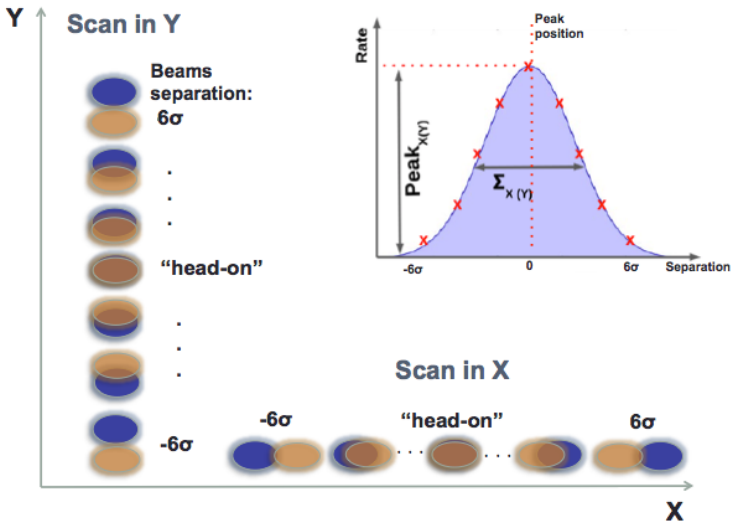
\includegraphics[scale=.37]{Chapter3/vdm_sketch.png}
    \caption[Sketch of a vdM scan in X and Y planes and example of fitting resulting rates]{ The sketch of a vdM scan in X and Y planes. The indent sketch is an example of the fitting of the resulting rates \cite{vdM_sketch}.}
    \label{vdm_sketch}
  \end{figure}
\end{center}
